\documentclass[border=6pt]{standalone}
\usepackage{tikz}
\usetikzlibrary{arrows.meta,positioning,fit,calc}
\definecolor{fg}{HTML}{3B3220}
\definecolor{fgbody}{HTML}{544736}
\definecolor{stroke}{HTML}{7A5A10}
\definecolor{surf}{HTML}{FAF6EE}
\definecolor{surfemph}{HTML}{F2E9D4}
\definecolor{surfact}{HTML}{F6E7E0}
\definecolor{bdim}{HTML}{CFC6B2}
\definecolor{bemph}{HTML}{7A5A10}
\definecolor{bact}{HTML}{8F1D1D}
\begin{document}
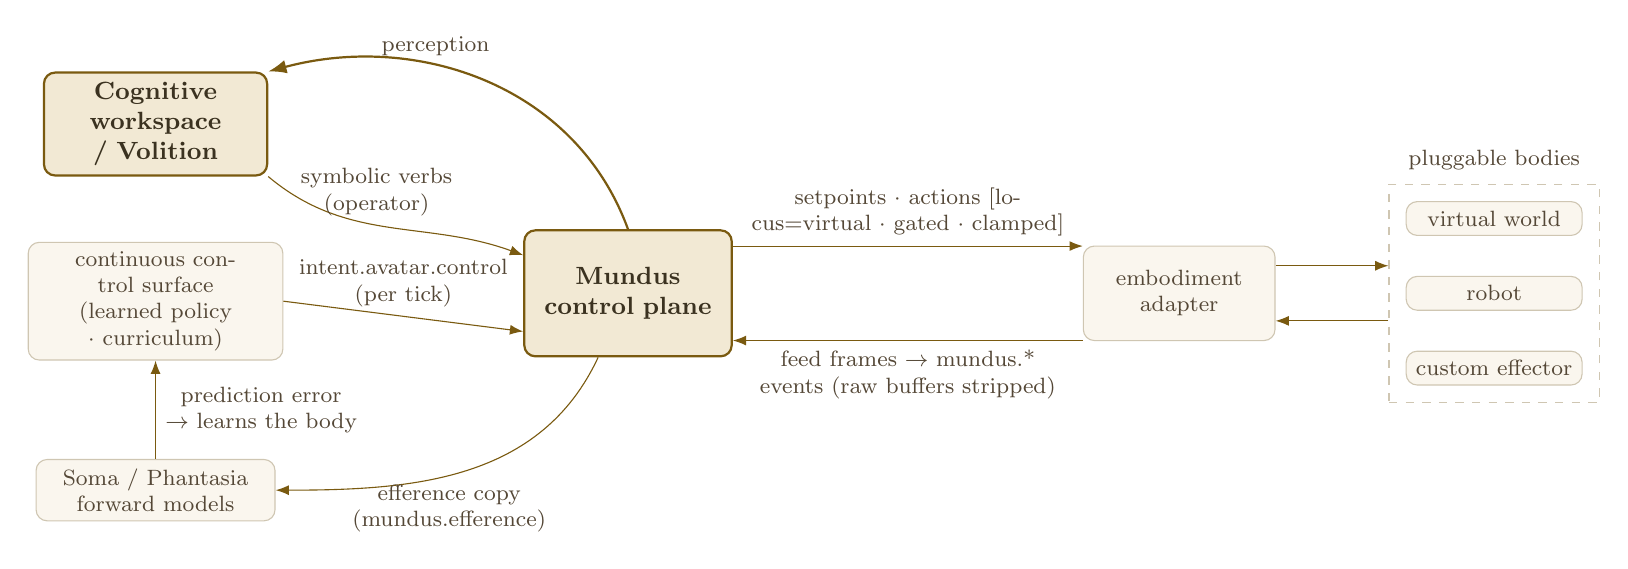
\begin{tikzpicture}[
  font=\small,>=Latex,
  mod/.style={draw=bdim, rounded corners, fill=surf, text=fgbody, align=center, font=\footnotesize},
  work/.style={draw=bemph, thick, rounded corners, fill=surfemph, text=fgbody, align=center},
  act/.style={draw=bact, rounded corners, fill=surfact, text=fgbody, align=center, font=\footnotesize},
  lbl/.style={font=\footnotesize, text=fgbody, align=center},
]
% central control plane
\node[work, text width=24mm, minimum height=16mm] (mundus) at (0,0)
  {\textcolor{fg}{\textbf{Mundus control plane}}};
% left column: workspace, control surface, forward models
\node[work, text width=26mm, minimum height=12mm] (ws) at (-6.0,2.15)
  {\textcolor{fg}{\textbf{Cognitive workspace / Volition}}};
\node[mod, text width=30mm] (ccs) at (-6.0,-0.1)
  {continuous control surface\\(learned policy $\cdot$ curriculum)};
\node[mod, text width=28mm] (fm) at (-6.0,-2.5)
  {Soma / Phantasia\\forward models};
% right: adapter and pluggable bodies
\node[mod, text width=22mm, minimum height=12mm] (adapter) at (7.0,0)
  {embodiment\\adapter};
\node[mod, text width=20mm] (b1) at (11.0,0.95) {virtual world};
\node[mod, text width=20mm] (b2) at (11.0,0.0)  {robot};
\node[mod, text width=20mm] (b3) at (11.0,-0.95) {custom effector};
\node[draw=bdim, dashed, fit=(b1)(b2)(b3), inner sep=6pt] (bodies) {};
\node[lbl, above=0.5mm of bodies] {pluggable bodies};

% --- perception: bodies -> adapter -> mundus -> workspace ---
\draw[->, draw=stroke] ([yshift=-3.5mm]bodies.west) -- ([yshift=-3.5mm]adapter.east);
\draw[->, draw=stroke] ([yshift=-6mm]adapter.west) --
  node[lbl, below, text width=38mm]{feed frames $\rightarrow$ mundus.* events (raw buffers stripped)} ([yshift=-6mm]mundus.east);
\draw[->, thick, draw=stroke] (mundus.north) to[out=110,in=15]
  node[lbl, above, pos=0.62]{perception} (ws.north east);

% --- action: workspace / control surface -> mundus -> adapter -> bodies ---
\draw[->, draw=stroke] (ws.south east) to[out=-40,in=160]
  node[lbl, above, pos=0.45]{symbolic verbs\\(operator)} (mundus.160);
\draw[->, draw=stroke] (ccs.east) --
  node[lbl, above]{intent.avatar.control\\(per tick)} (mundus.200);
\draw[->, draw=stroke] ([yshift=6mm]mundus.east) --
  node[lbl, above, text width=40mm]{setpoints $\cdot$ actions {[}locus=virtual $\cdot$ gated $\cdot$ clamped{]}} ([yshift=6mm]adapter.west);
\draw[->, draw=stroke] ([yshift=3.5mm]adapter.east) -- ([yshift=3.5mm]bodies.west);

% --- efference loop: mundus -> forward models -> control surface ---
\draw[->, draw=stroke] (mundus.245) to[out=-115,in=0]
  node[lbl, below, pos=0.55]{efference copy\\(mundus.efference)} (fm.east);
\draw[->, draw=stroke] (fm.north) --
  node[lbl, right]{prediction error\\$\rightarrow$ learns the body} (ccs.south);
\end{tikzpicture}
\end{document}
